\section{Spiking Neural Networks}

\begin{quote}
    `The brain computes! This is accepted as a truism by the majority
    of neuroscientists engaged in discovering the principles employed in the
    design and operation of nervous systems. What is meant here is that any
    brain takes the incoming sensory data, encodes them into various biophysical
    variables, such as the membrane potential or neuronal firing rates, and
    subsequently performs a very large number of illspecified operations,
    frequently termed computations, on these variables to extract relevant
    features from the input.'
    \begin{flushright}
        \textit{-- Christof Koch \\ Biophysics of Computation}
    \end{flushright}
\end{quote}

The mammalian nervous system is principally composed of neurons and glial cells.
Glial cells primarily perform supplementary roles in the function and processing
of data in the nervous system, but it is still not fully understood what further
role they play \autocite{walz_role_1989}. Neurons are less numerous in the
nervous system, and are chemically unique in their functioning in the body.

TODO: Levels of emulation pg.13 Bostrom and Sandburg Roadmap

\begin{figure}[h]
    \centering
    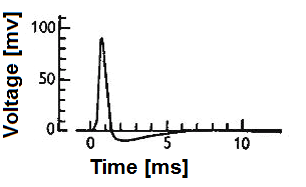
\includegraphics{figures/graphs/huxhog_spike.png}
    \DoubleCaption{The typical form of a neuronal action potential}
    {\small{Source: Nir.nossenson@wikipedia.com,
            \href{https://creativecommons.org/licenses/by-sa/4.0/deed.en}{CC BY-SA 4.0}}}
    \label{neuronalactionpotentialexample}
\end{figure}
\vspace{1ex}

Each neuron acts as a gate of sorts, holding or releasing its potential in
response to signals as part of a greater network of neurons. This release often
takes the form if a spike, as seen \ref{neuronalactionpotentialexample}.
Together, the neurons in these networks perform the signal processing and
routing that "computes" the many sensory inputs to the nervous system.
\autocite{koch_biophysics_2004}

While not all neurons are spiking neurons, it is the properties of spiking
neurons and the interactions between them that are the focus of this review and
ultimately this entire document.

\subsection{Hodgkin–Huxley model}

In 1952, Alan Hodgkin and Andrew Huxley described a model of the squid giant
axon that accurately reflects the both the chemical changes and the form of the
action potential spike in the axon. \autocite{hodgkin_quantitative_1952}

The strength of the Hodgkin–Huxley model is in its adaptability. Every change in
a neuron during a spike, be it chemical or physical, can be mapped across, and
more complex behaviour can be recreated in the model thanks to its basis in the
core chemistry of a neuron. However, this complexity is not without pitfalls as
the computational power required to simulate such advanced models is large
enough that it becomes unfeasible to simulate large networks.

\subsection{Faster neuron models for large scale computation}

While it can be desirable to accurately model and simulate the chemical
interactions between individual components of the nervous system, it is
computationally infeasible to do so on a scale similar to that of a real-world
system due to the computational complexity of the Hodgkin - Huxley equations.
Fortunately, as a network becomes larger, the exact mechanisms of its individual
components can be approximated, and faster activation or threshold functions
that perform similarly to real ones can be substituted.

One such example of a simple model of a spiking neuron is the Leaky Integrate
and Fire (LIF) neuron. It uses a simple threshold function to approximate the
action potential spike generation of a Hodgkin–Huxley neuron
\autocite{trappenberg_fundamentals_2009}. As this is a relatively simple
approximation, it is tempting to assume that such a model would prove inaccurate
for anything more than basic prototypes, however LIF models have been shown to
replicate spiking patterns of more complex models with a low margin of error,
provided the models are under natural conditions
\autocite{teeter_generalized_2018}. This document will go into more detail on
the equations and implementation of LIF neurons in Chapter 3, starting with
equation \eqref{eq:LIF_TC}.